\documentclass{beamer}
\mode<presentation>
 \usetheme{CambridgeUS}
%\usepackage{bussproofs}
%\usetheme{Singapore}
%\usecolortheme{lily}
  %%\usetheme{Logictheme} %nothing else
  %\setbeamertemplate{footline}[frame number]
  
%%\usepackage{bussproofs}
%%\usepackage[latin1]{inputenc} 
%%\newcommand{\mypause}{}
%%\newcommand{\mypause}{\pause}



\title[ERTMS in Real Time Maude]{Towards safety analysis of ERTMS/ETCS Level 2 \\ in Real-Time
  Maude}
\author[Monika Seisenberger]{Phillip James, Andrew Lawrence, \\ Markus Roggenbach, and {\bf Monika Seisenberger}}
\date[FTSCS 2015, Paris]{FTSCS 2015, Paris, 7 November 2015}
\institute[Swansea University]{Swansea Railway Verification Group,\\ supported by Siemens Rail Automation}

\usepackage{tikz}
\usepackage{graphicx}
\newcommand{\Red}{\mathbf{Red}}

\newtheorem{mydef}{Definition}
\newtheorem{myremark}{Remark}
\newcommand{\ednote}[1]{{\bf #1}}
\newcommand{\fig}[1]{Fig.~\ref{fig:#1}}
\newcommand{\Val}{{\rm Val}}
\newcommand{\unprime}{{\rm unprime}}
\newcommand{\Vars}{{\rm Vars}}


\newcommand{\rungStart}{
  %% Draw a -
  -- ++(2,0)
}

\newcommand{\contact}[1]{
  %% Draw a -
  -- ++(1,0)
  %% Draw ]
  +(-0.1, 0.5) -- +(0, 0.5) -- +(0, -0.5)  -- +(-0.1, -0.5)
  %% Move across
  ++(0.4, 0)
  %% Draw text above
  +(0,0.8) node{#1}
  %% Move across
  ++(0.4, 0)
  %% Draw [
  +(0.1, 0.5) -- +(0, 0.5) -- +(0, -0.5)  -- +(0.1, -0.5)
  %% Reset to current point
  ++(0, 0) --
  %% Draw a -
  ++(1,0) 
}


\newcommand{\closedContact}[1]{
  %% Draw a -
  -- ++(1,0)
  %% Draw ]
  +(-0.1, 0.5) -- +(0, 0.5) -- +(0, -0.5)  -- +(-0.1, -0.5)
  %% Move across
  ++(0.4, 0)
  %% Draw text above
  +(0,0.8) node{#1}
  %% Draw close i.e. /
  +(-0.2, -0.5) -- +(0.2, 0.5)
  %% Reset to current point (i.e. middle)
  ++(0, 0)
  %% Move across
  ++(0.4, 0)
  %% Draw [
  +(0.1, 0.5) -- +(0, 0.5) -- +(0, -0.5)  -- +(0.1, -0.5)
  %% Reset to current point
  ++(0, 0) --
  %% Draw a -
  ++(1,0) 
}

\newcommand{\coil}[1]{
   %% Draw a -
  -- ++(1,0)
  %% Move to end of -
  +(0.5,-0.5)
  %% Draw arc (
  arc (270:90:0.5cm)
  %% Move across
  ++(0.3, 0)
  %% Draw text above
  +(0,0.3) node{#1}
  %% Reset
  +(0.3,-1)
  %% Draw Arc )
  arc (-90:90:0.5cm)
  %% Move to center of )
  ++(0.5,-0.5)
  %% Finish Path
  ;
}


\newcommand{\nodeLink}[1]{
  %% Draw a -
  -- ++(0.5,0) node[inner sep=0pt, minimum size=0pt] (#1){};
}

\newcommand{\nodeLinkInline}[1]{
  %% Draw a -
  -- ++(0.5,0) node[inner sep=0pt, minimum size=0pt] (#1){} -- ++(0.5,0) 
}


\newcommand\boxAngle{150}

\newcommand{\mybox}[5]{ 
  %% #1 = Width, #2 = Height, #3 = Depth, #4 = x, #5 = y
  %% Front face
  \draw  (#4,#5) rectangle +(#1,#2);
  %% Draw side
  \draw [fill=gray!25] (#4,#5) -- ++(\boxAngle:#3) -- ++(0,#2) -- ++(\boxAngle:-#3);
  %% Draw top
  \draw [fill=gray!50] (#4,#5) ++(0,#2) -- ++(\boxAngle:#3) -- ++(#1,0) -- ++(\boxAngle:-#3);
}

\tikzstyle{myArrow}=[draw,->, line width=1.5pt]





\begin{document}

\begin{frame}
  \titlepage
\end{frame}


\begin{frame}

\frametitle{Overview:  ERTMS/ETCS in Real-Time
  Maude}

\medskip

\begin{center}
To investigate how a Centralized Traffic Control System, \\
the European Rail Traffic Management System (ERTMS) \\
can be modelled and verified using the Real-Time-Maude system
\end{center}
%\pause

\bigskip

Overview:

%\begin{itemize}
%  \item \underline{Part I:} ERTMS -- what it is
% \item \underline{Part II:} ERTMS -- how it works
%  \item \underline{Part III:} Generic Modelling: ERTMS as a hybrid automaton
%  \item \underline{Part IV:} Encoding in Real-Time Maude   
%  \item \underline{Part V:} Verification \& simulation results
%\end{itemize}

\begin{itemize}
 \item \underline{Part I:} ERTMS -- what it is 
  \item \underline{Part II:} ERTMS -- how it works
  \item \underline{Part III:} Modelling of ERTMS in Real-Time Maude   
  \item \underline{Part IV:} Validation
\item \underline{Part V: } Verification
\end{itemize}
%\begin{itemize}
 % \item \underline{Part I:} ERTMS -- what it is and how it works
  %\item \underline{Part II:} Modelling of ERTMS in Real-Time Maude   
  %\item \underline{Part III:} Validation and Verification results
%\end{itemize}

\bigskip

\end{frame}

\section{PART I: ERTMS -- what it is}

\begin{frame}
\begin{center}
{\Large ERTMS -- what it is and how it works}
\end{center}
\end{frame}



\begin{frame}

\frametitle{European Rail Traffic Management System (ERTMS) I}

What it is: 
\begin{itemize}

\item
European standard of signalling, control and train protection 
%Standard of signalling, control and train protection

\item
To replace the many incompatible safety systems (20!) currently used by
European railways

\item 
Offers possibility for traffic management

\item Originally designed for Europe, has rapidly become a global standard.
\end{itemize}

\bigskip

Some facts:
\begin{itemize}
\item Europe: Switzerland (1200km, full coverage by 2017), Denmark (4000km, full coverage by 2024), Germany, Belgium, Spain, Austria;  UK: First line in Wales: Cambrian Coast Line, 215km, Norway (80km)
  \item World wide: China: 8000km, Saudi Arabia, Turkey, 2000km, SA ...


%\item SA: Gautrain Rapid Rail Link, 80km 

%\item SA: Spoornet ORE Export Line -Sishen to Saldanha, 861km , freight train line.
\end{itemize}




\end{frame}



\begin{frame}

\frametitle{European Rail Traffic Management System (ERTMS) II}

Traditional railway interlockings control the rail traffic via signals. \\
In short:  ERTMS  removes the signals, and replaces them by communication between trains and interlockings.

\bigskip\bigskip

ERTMS  shall achieve:
\begin{itemize}

\item interoperability

\item ease of maintenance  (less track equipment) 

\item higher capacity \pause (40\%)\pause 

\end{itemize}

\bigskip\bigskip

Open research questions include:
\begin{enumerate}

\item
How can safety be verified? 

\item
How can capacity be measured and improved?

\item
How can reliability be measured and estimated?\pause

\end{enumerate}

Here: 1 and, partially, 2.

\end{frame} 

\section{Part II: ERTMS -- how it works}

%\begin{frame}
%\begin{center}
%{\Large ERTMS -- how it works}
%\end{center}
%\end{frame}


\begin{frame}
\frametitle{System components of ERTMS, level 2}
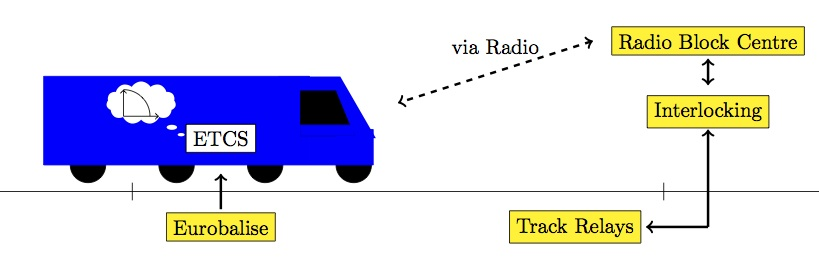
\includegraphics[scale =0.8]{ETCSlevel2}

\bigskip

Main Responsibilities:\\

Trains - communicate position/speed, and receive movement authorities.\\
RBC - grants MAs/denies MA requests, consults with Interlocking
   Interlocking  - allows for setting new routes, responsible for safety.\\  \pause
Controller (not in picture) - requests new routes.


\end{frame}



\begin{frame}
\frametitle{Information flow in ERTMS, level 2}
\begin{center}
\includegraphics[scale=0.5]{architecture.png}
\end{center}
\end{frame}






\section{PART III: Modelling of  ERTMS in Real-Time-Maude}

\begin{frame}
\begin{center}{\Large Modelling of ERTMS in Real-Time-Maude}
\end{center}
\end{frame}


\begin{frame}[fragile]
%\frametitle{ Real-Time-Maude (Peter \"Olveczky, Jos\'e Meseguer 2002) }
\frametitle{ Object Oriented Modelling in Real-Time-Maude}

%Real-Time Maude (Peter C. \"Olveczky and Jos\'e Meseguer 2002) is a language and tool extending Maude, 

- Real-Time-Maude allows for simulation and formal analysis of real-time and hybrid systems.

\bigskip

- Object based systems are modelled as multisets of objects and messages of a sort \texttt{Configuration}, a subset of Maude's built-in in sort System. 

\bigskip

 - A real-time specification consists of
\begin{itemize}
\item the sort \verb|Time| (in our case \verb|PosRat|), 
\item the constructor \verb| {_} : System -> Globalsystem|
\item instantaneous rewrite rules, 
\item a so-called tick rule that defines how time elapses.
\end{itemize}



\begin{verbatim}
crl [tick] : {CURRENT} => {delta(CURRENT,R)} in time R 
                if R <= mte(CURRENT) [nonexec] .
\end{verbatim}

where 
\verb|delta|  defines the effect of time elapse on a configuration.\\
\quad \qquad \verb|mte| defines the maximal possible time elapse.


\end{frame}






\begin{frame}[fragile]
\frametitle{Modelling 1:  location specific data \& messages}

Encoding of the rail topology:
\begin{verbatim}
sort RouteName . ops RouteName1A ... : -> RouteName .
sort Track .     ops AA AB AC ... : -> Track        .
sort Point .     ops P1 P2 : -> Point               . 
\end{verbatim}

\bigskip

Messages to be exchanged between the ERMTS components:
\begin{verbatim}
msg routerequest : RouteName -> Msg . 
msg marequest : Oid Track -> Msg .
\end{verbatim}

\end{frame}

\begin{frame}[fragile]
\frametitle{Modelling 2: Instantaneously reacting sub-systems}

No time-constraints:
\begin{verbatim}
eq mte(< O1 : Controller | >) = INF .
\end{verbatim} 

Interlocking -- a class with internal states:
\begin{verbatim}
class Inter |  routeset : MapRouteName2Bool, 
               pointslocked : MapPoint2Bool,
               occ : MapTrack2Bool, 
               pointPositions : MapPoint2PointPos  .
\end{verbatim}

Ignoring a route request:
\begin{verbatim}
crl  routerequest(RN1) 
     < O : Inter |  occ : MAPTB1, pointslocked : MAPPB3 >
     => 
     < O : Inter | > if (not checkClear(RN1, MAPTB1)) or 
                             pointsLocked(RN1, MAPPB3) .
\end{verbatim}

\end{frame}



\begin{frame}[fragile]
\frametitle{Modelling 3: Trains with ERTMS equipment} 
\begin{verbatim}
 crl [acc] :
  ...
  delta(< O : Train | state : acc, dist : DT, speed : S, 
           ac : A, ma : MA , tseg : AN, maxspeed : MAX >, R)
  =>
  ... 
  < O : Train | state : if (S + R * A == MAX)     
                        then cons 
                        else (if R == mteMA(DT,S,A,MA)
                               then brake
                               else acc fi) fi, 
                 dist : DT + S * R + R * R * A * 1/2,
                 speed : S + A * R > )
                                         if not AN == Exit .
\end{verbatim}      
\end{frame}



\begin{frame}
\frametitle{Modelling 3:  Trains with ERTMS equipment}
\begin{center}
\includegraphics[scale=0.55]{trainautomaton}
\end{center}
\end{frame}





\section{Part IV: Validation through Simulation and Error injection}

\begin{frame}
\begin{center}
{\Large Validation \& Verification}
\end{center}
\end{frame}


\begin{frame}
\frametitle{Validation through Simulation}
We have validated our model through exploring various train movements.\\ \quad \\

For example, rewriting a train starting on track AA: \\ \quad \\ 
\texttt{ \small{
(trew \{ 
  < inter1 : Inter | pointPositions : (P1 |-> normal,
                                       P2 |-> normal) , ... >
  < train1 : Train | state : acc, dist : 2, speed : 0, ac : 1, 
                     ma : 1498, tseg : AA , maxspeed : 60 > \}
in time <= 39 .)\\ \quad \\
}}
shows that it accelerates until it is required to begin braking due to its MA:\\ \quad \\

\texttt{\small{
 ... < train1 : Train | ac : 1, dist : 1499446241/2000000,
    ma : 1498, maxspeed : 60, speed : 38671/1000, 
    state : brake, tseg : AA >... in time 38671/1000
}}

\end{frame}

\begin{frame}
\frametitle{Validation through Simulation (2)}
It then makes a movement authority request: \\ \quad \\

\texttt{ \small{marequest(train1,AA) < inter1 : ...> 
 < train1 : Train | speed : 37671/1000, ... > in time 39671/1000
}}\\ \quad \\

However at this point the system will not progress until we add an RBC to deal with the request... See the paper for the complete example!

\end{frame}

\begin{frame}
\frametitle{Error Injection: Train - Incorrect  braking parameters}
Our modelling is able to find errors, for example:
\begin{center}
Decelleration for used for computation: 1; physical deceleration: 8/10.
\end{center}

\texttt{\small {< train1 : Train | ...  dist : 3249, ac : 1, ma : 6499, tseg : AD , maxspeed : 20 >
    < train2 : Train |  ... ac : 8/10, ma : 1, tseg : Entry , maxspeed : 60 > ...}}

\bigskip

Model checking is able to produce a couter example
\bigskip

\texttt{\small{< train1 : Train | ac : 1,dist : 15662341/2500,ma : 6499,
      maxspeed : 20,speed : 20,state : cons,tseg : AF >
    < train2 : Train | ac : 4/5,dist : 968593576867/156250000,
      ma : 7999,maxspeed : 60,speed : 60,state : cons,
      tseg: AF > ...}}
\end{frame}

\begin{frame}
\frametitle{Error Injection: RBC Design Error}
Our modelling is able to find errors, for example:

\begin{center}
Assume the RBC is designed with incorrect EoA values, \\e.g. EoA of Route 1A = 3449m
\end{center}

Model checking is able to produce a couter example where train 1 ovveruns and hence is able to get within 100m of train 2:\\ \quad \\
\texttt{
...< train1 : Train | ac : 1,dist : 3449,ma : 3449,
      maxspeed : 20,speed : 0,state : stop,tseg : AD >}\\
\texttt{
< train2 : Train | ac : 1,dist : 12433788921/4000000,
      ma : 6499,maxspeed : 60, speed : 60,state : cons,
      tseg : AC > ...
}
\end{frame}


\section{Part V: Verification through Modellchecking}


\begin{frame}
\frametitle{Safety Verification through
  Model-checking}
Verification that trains cannot be within 100 metres of each other, e.g.:
\begin{center}
\texttt{
mc initState |=t [] nocrashDistance(train1,train2) . 
}
\end{center}
\begin{table}
\centering
{\footnotesize
  \begin{tabular}{|l|c|c|}
    \hline 
    \textbf{Scheme Plan} & \textbf{Round Robin Controller} &
    \textbf{Random Controller} \\
    & \textbf{Unbounded} & \textbf{in Time 300} \\
    \hline \hline
    Junction  & 2.4s / 5,767,435 rewrites & \hphantom{1}268.3s / 208,715,358 rewrites \\
    Pass-through Station & 3.0s  / 7,135,987 rewrites & \hphantom{1}439.2s / 308,629,500 rewrites \\
    Three Platform Station & 2.8s / 6,624,578 rewrites & 2697.1s / 729,201,878 rewrites \\
    \hline
 \end{tabular}
}
\caption{Verification results of model checking three scheme plans.}
\end{table}


\end{frame}

\section{Conlusion \& Future Work}

\begin{frame}
\begin{center}
{\Large Conclusion \& Future Work}
\end{center}
\end{frame}

\begin{frame}
\frametitle{Summary}

The firsts:
\begin{itemize}
\item First use of Maude / Real-Time Maude in the railway domain.
\item First formal model comprising of all ERTMS subsystems required
  for the control cycle.
\end{itemize}

The quality jump: 
\begin{itemize}
\item Rail control modelled as a hybrid system.
\item Safety properties in physical rather than in logical terms.
\end{itemize}

The verification results:
\begin{itemize}
\item Unrestricted controller: time bounded model-checking.
\item Restricted controller: unbounded model-checking.
\end{itemize}
\end{frame}

\begin{frame}
\frametitle{Future Work}

Further experiments:
\begin{itemize}
\item More, and more complex rail-yards.
\end{itemize}

Improving the models:
\begin{itemize}
\item Bi-directional rail-yards.
\item Further controller strategies. 
\item More complex train progression behaviour.
\end{itemize}

Reflecting on the models:
\begin{itemize}
\item Include further safety properties.
\item Address completeness.
\item Develop abstractions to increase in verification speed.
\end{itemize}

\end{frame}

\begin{frame}
\frametitle{Related work}

ERTMS is a complex systems of systems -- many focus on one subsystem only:
\begin{itemize}
\item
Vu et al.: Interlocking 
\item
Cimatti et al.: subsystem for allocation of logical routes to trains
\item
Nardone et al.: radio block centre.
\end{itemize}

Our objective: verify location specific data -- others work towards:
\begin{itemize}
\item Software model checking of subsystems.
\item System testing.
\item Check the consistency of the ERTMS specifications themselves.
\end{itemize}

We verify system parameters on the \emph{design level} -- others focus on
verification of the \emph{implementation}.

\end{frame}

\end{document}




\end{document}

\section{}


\begin{frame}
\frametitle{Ongoing work: Modelling and Verification}
\begin{itemize}
\item Modelling of  the controller: \\
Knows of trains routes, max speed of each train, initializes trains.\\
$\to $ Route setting, interaction with interlocking.\\


\bigskip
\item Generic track plans, control tables, release tables. 



\bigskip

\item Scenarios that lead to counter examples.

\bigskip
\item Limits of Model checking.

\bigskip

\item Review of assumptions: maximal progress assumption.

\bigskip

\item Completeness of modelling approach
\end{itemize}

\end{frame}


%\begin{frame}
%\frametitle{Modelling of a  simple Controller}
%Controller currently acts as scheduler for second example. Class with three parameters: 
%\begin{itemize}
%\item \texttt{trainorder}: stores a list of trains that are going to enter the track.

%\item \texttt{trainmax}: stores the maximum speed for each train.

%\item \texttt{trainroute}: stores the route of each train. 
%\end{itemize}

%\bigskip
%The controller sends request messages to the rbc that allows the train to enter.
%If granted, the train is removed from \texttt{trainorder}, and a train object is generated.
%A message is sent to the interlocking that the initial trainsegement is occupied.
%\end{frame}






\begin{frame}
\frametitle{Conclusion \& Future Work}


\begin{itemize}
%\item Demonstrated various techniques to verify  and simulate Railway control systems.



\item Our modelling approach works and is rich enough it to analyze ERTMS for
  important safety and capacity properties.

\item Real-Time Maude offers a competitive framework for modelling \&
 analysing ERTMS.
\medskip

%\item Extracted a SAT solver, sound and complete.
%\item Demonstrated that efficiency considerations can be taken into account at the proof level.

\end{itemize} %\pause


Future Work:
\begin{itemize}
%\item Formalize the relation between hybrid automaton and its discrete
%  approximation in Real-Time Maude.


\item Enrich the modelling to capture more aspects of ERTMS.
\item Develop the timed simulations towards capacity measures.


\bigskip

\item Aside: Final year student - Automatic translation of Ladderlogic into Real-Time Maude

%\item Further optimize the extracted SAT solver; takle a different class of problems.

\end{itemize}

\end{frame}

\end{document}
\begin{frame}
\frametitle{References}    
 
%Specification Implementation Verification Method:

  \begin{thebibliography}{10}    
  \beamertemplatearticlebibitems
  \bibitem{} James, P., Lawrence, A.,  Moller, F., Roggenbach, M., Seisenberger, M. and Setzer, A.Chadwick, S. ,P. Kanso, K., :
\newblock{\em  Verification of solid state interlocking programs.}
\newblock In SEFM'13, LNCS 8368, Springer 2014.
\end{thebibliography} 

\bigskip
%Extraction of SAT and Resolution algorithm:

\begin{thebibliography}{10}    
  \beamertemplatearticlebibitems
  \bibitem{}
    Berger, U.,  Lawrence, A., Nordvall Forsberg, F. , Seisenberger, M. 
    \newblock {\em Extraction of Verified Decision Procedures}. LMCS, to appear. 

\bigskip

\bibitem{} Lawrence, A, Berger, U. , James, P., Roggenbach, M., Seisenberger, M.
\newblock {\em Modelling and Analysing the European Rail Traffic Control System}
\newblock FTSCS, 2014.

\end{thebibliography}
\end{frame}



\end{document}

\begin{frame}

\frametitle{European Rail Traffic Management System (ERTMS) II}

Formal methods and ERTMS:
\begin{itemize}

\item
EuRailCheck (2009): \\ suggested methodology and tools for
formalization and validation of the standard.

\item
Open ETCS Project (ongoing): \\ works towards an integrated framework for
modelling, development, implementation and testing of the standard.

\end{itemize}

Open research questions include:
\begin{enumerate}

\item
How can safety be verified? 

\item
How can capacity be measured and improved?

\item
How can reliability be measured and estimated?

\end{enumerate}

Here: 1 and, partially, 2.

\end{frame}

\section{Modelling and Analyzing ERTMS}

%\begin{frame}
%\begin{center}
%{\Large ERTMS -- how it works}
%\end{center}
%\end{frame}

\begin{frame}
\frametitle{Data in the ERTMS, level 2}
\begin{itemize}
\item Trains send position and speed (continuous data) and request \alert{Movement Autorities} from the RBC.

 
\item The radio block processor (RBC) consults with the interlocking and
grants or denies  a \alert{movement
  authority} (MA).

\medskip

\item The MA consists of a position on the track past which the train cannot
proceed called the end of authority (EoA) [and a static speed profile].

\medskip

\item Trains move on the track according to the physical laws of movement,
their breaking is controlled against a differential equation, their
acceleration follows a differential equation.

\medskip

\item Together the RBC, trains and the interlocking form a \alert{hybrid
  system}.
 \end{itemize}
\end{frame}


\begin{frame}
\frametitle{Object Oriented Modelling in  Real-Time Maude}

Real-Time Maude (Peter C. \"Olveczky and Jos\'e Meseguer 2002) is a language and tool extending Maude, 
that allows for simulation and formal analysis of real-time and hybrid systems.

\medskip



We make use of especially of its
\begin{itemize}

\item OO features

\item \alert time rewriting rules:
%
\begin{flushleft}
\texttt{  rl  [label] : \{Sys\} => \{Sys\} in time t .}\\
\texttt{  crl [label] : \{Sys\} => \{Sys\} in time t if C .} 
\end{flushleft}

%\item $\delta$ operator %describes system evolution in one time unit


\end{itemize}
\end{frame}
\begin{frame}[fragile]
\frametitle{Object Oriented Modelling}
\begin{verbatim}
mod CONFIGURATION is  
    *** basic object system sorts  
    sorts Object Msg Configuration .  
 
    *** construction of configurations  
    subsort Object Msg < Configuration .  
    op none : -> Configuration [ctor] .  
    op __ : Configuration Configuration -> Configuration  
         [ctor config assoc comm id: none] .
\end{verbatim}
\end{frame}

\begin{frame}[fragile]
\frametitle{Timed Progress of a train in state ``accelerating''}
\begin{verbatim}
crl [incspeed] : 
  {delta(< O : Train | state : acc, dist : DT, speed : S, 
                       ac : A, ma : MA, maxspeed : MAX >)
           REST}

   => 

  {pos(O,DT) 
   < O : Train |  dist : (DT + S), speed : S + A > 
   REST
  } 
  if S + A < MAX and ... .
\end{verbatim}
\end{frame}



\begin{frame}[fragile]
\frametitle{Message consumption for the RBC in state ``wait''}
\begin{verbatim}
rl [rbcgrant]:
  { grant(N) 
    <O : RBC | state : wait, lasttrain : T1, ma : MAP1 > 
    REST
  } 

=>

  { <O : RBC | state : rbcidle, 
               ma : insert(T1,endoftrack(N),MAP1) >
    grantma(T1, endoftrack(N)) 
    REST
  } .
\end{verbatim}
\end{frame}




\begin{frame}[fragile]
\frametitle{$\delta$ operator -- by {\"O}lveczky and Thorvaldsen, 2007}

\begin{verbatim}
op delta : Configuration -> Configuration . 
vars CON CON1 CON2 : Configuration . 
var OCREST : ObjectConfiguration .


rl [timetrans] : {OCREST} => {delta(OCREST)} in time 1 .
rl [delta] : delta(CON1 CON2) => delta(CON1) delta(CON2) .

--- mte = maximal time elapse
rl [mte] : {CON} => {delta(CON)} in time 1 if mte (CON) >= 1 .  

eq mte(none) = INF 
eq mte(CON1 CON2) = min(mte(CON1), mte(CON2)).
eg mte (MSG) = 0
eg mte (<    >) = ....
\end{verbatim}
\end{frame}
\begin{frame}[fragile]
\frametitle{Modelling 3: Trains with ERTMS equipment} 
\begin{verbatim}
 crl [acc] :
   < O1 : Inter | pointPositions : PointSettings >
   delta(< O : Train | state : acc, dist : DT, speed : S, 
            ac : A, ma : MA , tseg : AN, maxspeed : MAX >, R)
   =>
   < O1 : Inter | > 
   trackseg(PointSettings, 
   < O : Train | state : if (S + R * A == MAX)     
                         then cons 
                         else (if R == mteMA(DT,S,A,MA)
	                               then brake
                               else acc fi) fi, 
                  dist : DT + S * R + R * R * A * 1/2,
                  speed : S + A * R > )
    if not AN == Exit .
\end{verbatim}      
\end{frame}
\end{document}
